\documentclass[10pt,a4paper]{article}
\usepackage[a4paper, margin=2cm]{geometry}
\usepackage{needspace}
\usepackage[nobottomtitles]{titlesec}
\usepackage{multicol}
\usepackage{xcolor}
\usepackage{fp}
\usepackage{xfp}
\usepackage{numprint}
\usepackage{siunitx}
\usepackage{enumitem}
\usepackage[version=4]{mhchem}
\usepackage{chemfig}
\usepackage{mol2chemfig}
\usepackage{WriteOnGrid}
\usepackage{frcursive}
\usepackage{csvsimple}%

\DeclareSIUnit{\nothing}{\relax}

\newcommand{\element}[1]{%
    \par\noindent%
    \rule{\textwidth}{0.4pt}\par%
    \smallskip%
    
    \par\noindent%
    \rule{\textwidth}{0.4pt}\par%
    \medskip%
}

\newcommand{\scoring}[1]{{\tiny (#1)}}

% Commandes pour les réponses avec gestion des arguments optionnels
\newcommand{\mauvaise}[2][]{
    \item{Mauvais: [#1] #2}
}
\newcommand{\bonne}[2][]{
    \item{Bonne: [#1] #2}
}

\newenvironment{question}[1]{
    \par\noindent
    \textbf{Question #1:} \\ \smallskip
}{\newline}

\newenvironment{questionmult}[1]{
    \par\noindent
    \textbf{Question #1:} \\ \smallskip
}{\newline}

\newenvironment{reponses}{
    \\
    \smallskip
    \begin{itemize}
}{\end{itemize}\smallskip}

\newenvironment{reponseshoriz}{
    \\
    \smallskip
    \begin{tabular}{l}
}{\end{tabular}\smallskip}

\newcommand{\explain}[1]{\\ \textcolor{red}{#1}}

\begin{document}

\section{Stéréochimie et réactions acido-basiques de l'ibuprofène}
\textbf{Source du sujet :} Baccalauréat de mars 2021

\subsection{Introduction}
Au XIX\textsuperscript{e} siècle, on utilisait déjà des principes actifs chiraux comme la morphine, administrée comme
anti-douleur. Malgré les idées énoncées par Pasteur à la fin du XIXtextsuperscript{e} siècle, les chimistes ont
mis beaucoup de temps pour comprendre que la chiralité pouvait avoir un impact considérable sur
les organismes vivants. Cette prise de conscience a eu lieu dans les années 1960 avec le drame de
la thalidomide, médicament qui fut administré aux femmes enceintes comme anti-vomitif, et qui
provoqua chez les nouveau-nés de graves malformations. On connaît aujourd'hui la raison de ce drame~:
alors que l'énantiomère $R$ est bien anti-vomitif, l'énantiomère $S$ est tératogène*.

L'ibuprofène est connu pour avoir un effet biologique anti-inflammatoire et antipyrétique sous sa
forme $S$ et sans effet thérapeutique notable sous sa forme $R$. Le produit commercial est généralement
le mélange racémique**. Cependant, seul l'énantiomère $S$ est biologiquement actif et présente les effets
thérapeutiques désirés. L'énantiomère $R$ est très difficile à séparer du $S$, mais est heureusement
inoffensif. L'énantiomère $S$ seul commence à produire son effet 12 minutes après son absorption,
alors que le mélange racémique n'est actif que 38 minutes après avoir été absorbé. Très curieusement,
le corps humain possède la propriété de pouvoir transformer chimiquement l'énantiomère $R$ inactif en
énantiomère $S$.

\textit{*tératogène : peut provoquer des malformations fœtales}

\textit{**Quand un mélange contient en proportion égale les deux énantiomères $R$ et $S$
d'une molécule ayant un seul carbone asymétrique, le mélange est qualifié de racémique.}

\subsection{Données}
\begin{itemize}
    \item Numéros atomiques : $Z(H) = 1$~; $Z(C) = 6$~; $Z(O) = 8$.
    \item pKa du couple acide/base de l'ibuprofène : $pKa = 4,5$ à $\SI{20}{\degreeCelsius}$.
\end{itemize}

\begin{center}
\chemfig{
OH-[:210,,1](=[:270]O)-[:150](\mcfatomno{*}-[:90]CH3)-[:210]=_[:270]-[:210]=_[:150](-[:90]%
=_[:30]-[:330])-[:210]-[:150](-[:210])-[:90]
}
\par\noindent\small\textit{Structure de l'ibuprofène}
\end{center}

\begin{center}
\chemfig{
-[:210]=_[:270]-[:210]=_[:150](-[:90]%
=_[:30]-[:330])-[:210]-[:150](-[:210])-[:90]
}
\par\noindent\small\textit{Le groupe ci-dessus, pourra être noté MPP pour méthyl phénylpropane,
il peut simplifier vos représentations}
\end{center}

\subsection{Questions}

\begin{questionmult}{ibuprofene1}
    Représenter la formule topologique de l'ibuprofène.
    \begin{EnvQuadrillage}[NbCarreaux=20x4,Grille=Seyes,Marge=1]
    \end{EnvQuadrillage}
    \AMCOpen{}{
        \mauvaise[F]{NA}\scoring{b=0}
        \mauvaise[X]{Partiellement correct}\scoring{b=1}
        \bonne[C]{Formule correcte}\scoring{b=2}
    }
    \explain{
        La formule topologique de l'ibuprofène était donnée dans le sujet.
        Il est possible de simplifier son écriture en utilisant le groupe MPP~:
        \chemfig{
        -[:210]=_[:270]-[:210]=_[:150](-[:90]%
        =_[:30]-[:330])-[:210]-[:150](-[:210])-[:90]
        }  \chemfig{OH-[:210,,1](=[:270]O)-[:150](\mcfatomno{*}-[:90]CH3)-[:210]MPP}
    }
\end{questionmult}

\begin{questionmult}{ibuprofene2}
    Entourer, sur la formule topologique (que vous avez dessiné au dessus), le groupe caractéristique présent dans la molécule
    d'ibuprofène et nommer la famille fonctionnelle associée.
    \begin{EnvQuadrillage}[NbCarreaux=20x2,Grille=Seyes,Marge=1]
    \end{EnvQuadrillage}
    \AMCOpen{}{
        \mauvaise[F]{NA}\scoring{b=0}
        \bonne[A1]{Groupe identifié}\scoring{b=1}
        \bonne[A2]{Famille nommée}\scoring{b=1}
    }
    \explain{
        Le groupe caractéristique est le groupe carboxyle ($-COOH$), situé à l'extrémité de la chaîne carbonée.
        Ce groupe définit la famille fonctionnelle des acides carboxyliques.
    }
\end{questionmult}

\begin{questionmult}{ibuprofene3}
    Justifier que l'atome de carbone noté C* dans la représentation de la molécule d'ibuprofène est asymétrique.
    \begin{EnvQuadrillage}[NbCarreaux=20x2,Grille=Seyes,Marge=1]
    \end{EnvQuadrillage}
    \AMCOpen{}{
        \mauvaise[F]{NA}\scoring{b=0}
        \bonne[A1]{Bases}\scoring{b=1}
        \bonne[A2]{Justification correcte}\scoring{b=1}
    }
    \explain{
    Le carbone $C^*$ est asymétrique car il est lié à quatre groupes d'atomes différents~:
    \begin{itemize}
        \item Un groupe carboxyle ($-COOH$).
        \item Un atome d'hydrogène ($-H$) (omit dans la représentation topologique).
        \item Un groupe méthyle ($-CH_3$).
        \item Un groupe phényle (représenté par $MPP$).
    \end{itemize}
    }
\end{questionmult}

\begin{questionmult}{ibuprofene4}
    La représentation d'un des énantiomères A de l'ibuprofène est donnée ci-dessus. Représentez,
    en perspective de Cram, l'autre énantiomère B de l'ibuprofène.
    \centering
    \chemfig{ CH_3>[:100](<:[:-30]H)(-[90]COOH)-[:210]MPP }
    \par\noindent\small\textit{Énantiomère A}
    \begin{EnvQuadrillage}[NbCarreaux=20x4,Grille=Seyes,Marge=1]
    \end{EnvQuadrillage}

    \AMCOpen{}{
        \mauvaise[F]{NA}\scoring{b=0}
        \bonne[A1]{Cram perspective}\scoring{b=1}
        \bonne[A2]{Représentation correcte}\scoring{b=1}
    }
    \explain{
        Pour représenter l'énantiomère B en perspective de Cram~:
        \begin{itemize}
            \item Inverser la position des groupes autour du carbone asymétrique.
            \item Le groupe $CH_3$ et l'atome d'hydrogène $H$ échangent leurs positions par rapport à l'énantiomère A.
        \end{itemize}
        Note~: n'importe quelle inversion de groupes autour du carbone asymétrique donne l'autre énantiomère.
        \chemfig{ H>[:100](<:[:-30]CH_3)(-[90]COOH)-[:210]MPP }
    }
\end{questionmult}

\begin{questionmult}{ibuprofene5}
    Déterminer la configuration absolue, R ou S, de chaque énantiomère A et B en expliquant votre démarche.
    \begin{EnvQuadrillage}[NbCarreaux=20x6,Grille=Seyes,Marge=1]
    \end{EnvQuadrillage}
    \AMCOpen{}{
        \mauvaise[F]{NA}\scoring{b=0}
        \bonne[A1]{Raisonnement}\scoring{b=1}
        \bonne[A2]{Résultat}\scoring{b=1}
    }
    \explain{
    La configuration absolue est déterminée en utilisant les règles Cahn-Ingold-Prelog~:
    \begin{itemize}
        \item Classer les groupes liés au carbone asymétrique par ordre de priorité (numéro atomique décroissant).
        \item Orienter la molécule de sorte que le groupe de plus faible priorité soit dirigé vers l'arrière.
        \item Si les trois groupes restants sont ordonnés dans le sens horaire, la configuration est $R$. Sinon, elle est $S$.
    \end{itemize}
    Note: le \ce{C} lié à un \ce{O} (dans \ce{COOH}) est prioritaire sur le \ce{C} lié à un autre \ce{C} (dans \ce{MPP})
(   car \ce{_{8}O} est plus grand que \ce{_{6}C}), qui est prioritaire sur le \ce{C} lié à un \ce{H} (dans \ce{CH3}).
    \begin{center}
    \begin{minipage}[t]{0.45\textwidth}
        \centering
        \chemfig{ ^{\color{blue}3}CH_3>[:100]^{\color{blue}*}(<:[:-30]^{\color{blue}4}H)(-[90]_{\color{blue}1}COOH)-[:210]MPP^{\color{blue}2} } \\
        \noindent\small\textit{A: Énantiomère S}
%        \par\noindent\small\textit{A: Énantiomère S}
    \end{minipage}%
    \hspace{0.05\textwidth}% Espace entre les deux molécules
    \begin{minipage}[t]{0.45\textwidth}
        \centering
        \chemfig{ ^{\color{blue}4}H>[:100]^{\color{blue}*}(<:[:-30]^{\color{blue}3}CH_3)(-[90]_{\color{blue}1}COOH)-[:210]MPP^{\color{blue}2} } \\
        \noindent\small\textit{B: Énantiomère R}
%        \par\noindent\small\textit{B: Énantiomère R}
    \end{minipage}
    \end{center}
    }
\end{questionmult}

\begin{questionmult}{ibuprofene6}
    Expliquer en quoi un mélange racémique dans le cas de l'ibuprofène~:
    \begin{itemize}
        \item n'est pas dangereux pour les humains~;
        \item retarde son action par rapport à l'énantiomère S seul.
    \end{itemize}
    \begin{EnvQuadrillage}[NbCarreaux=20x4,Grille=Seyes,Marge=1]
    \end{EnvQuadrillage}
    \AMCOpen{}{
        \mauvaise[F]{NA}\scoring{b=0}
        \bonne[A1]{Racémique}\scoring{b=.5}
        \bonne[A2]{Dangereux}\scoring{b=.5}
        \bonne[A3]{Retarde}\scoring{b=.5}
        \bonne[A4]{Overall}\scoring{b=.5}
    }
    \explain{
    \begin{itemize}
        \item Le mélange racémique n'est pas dangereux car l'énantiomère $R$ est inactif, mais sans danger pour le corps humain.
        \item L'action est retardée car le corps doit convertir l'énantiomère $R$ en $S$ par une réaction enzymatique, ce qui prend environ 38 minutes.
    \end{itemize}
    }
\end{questionmult}

\begin{questionmult}{ibuprofene7}
    L'ibuprofène est un acide faible. Il appartient à un couple acide-base de pKa égal à 4,5 à
    $\SI{20}{\degreeCelsius}$.
    \begin{enumerate}
        \item   Écrire la formule semi-développée de la base conjuguée de l'ibuprofène en notant MPP
                le groupe méthyl phénylpropane.
        \item   Indiquer si la forme basique de l'ibuprofène possède les mêmes propriétés
                stéréochimiques que la forme acide.
    \end{enumerate}
    \begin{EnvQuadrillage}[NbCarreaux=20x8,Grille=Seyes,Marge=1]
    \end{EnvQuadrillage}
    \AMCOpen{}{
        \mauvaise[F]{NA}\scoring{b=0}
        \bonne[A1]{Formule $\approx$}\scoring{b=.5}
        \bonne[A2]{Formule correcte}\scoring{b=.5}
        \bonne[B1]{Propriétés $\approx$}\scoring{b=.5}
        \bonne[B2]{Propriétés stéréochimiques}\scoring{b=.5}
   }
    \explain{
    \begin{itemize}
        \item Formule semi-développée de la base conjuguée de l'ibuprofène~: \ce{MPP-CH2-COO-}.
        \item La base conjuguée de l'ibuprofène conserve le carbone asymétrique dans la
         même chiralisme, donc elle possède les mêmes propriétés stéréochimiques que
         la forme acide.
    \end{itemize}
    }
\end{questionmult}

\begin{questionmult}{ibuprofene8}
    Écrire l'équation de la réaction acide-base dont la constante d'acidité Ka de ce couple acide-base
    est la constante d'équilibre.
    \begin{EnvQuadrillage}[NbCarreaux=20x2,Grille=Seyes,Marge=1]
    \end{EnvQuadrillage}
    \AMCOpen{}{
        \mauvaise[F]{NA}\scoring{b=0}
        \bonne[A1]{Formule $\approx$}\scoring{b=1}
        \bonne[A2]{Équation correcte}\scoring{b=1}
    }
    \explain{
    L'équation de la réaction acide-base est~:
    \begin{itemize}
        \item \ce{MPP-CH2-COOH + H2O <=> MPP-CH2-COO- + H3O+}.
        \item \ce{MPP-CH2-COOH} est l'acide.
        \item \ce{MPP-CH2-COO-} est la base conjuguée.
        \item \ce{H2O} et \ce{H3O+} forment le couple acide/base de l'eau.
    \end{itemize}
    }
\end{questionmult}

\begin{questionmult}{ibuprofene9}
    Indiquer sous quelle forme (acide ou basique) se trouve le principe actif d'un comprimé d'ibuprofène dans
    l'estomac de pH égal à environ 2, puis dans le sang de pH proche de 7,4. Un diagramme
    de prédominance légendé est accepté.
    \begin{EnvQuadrillage}[NbCarreaux=20x4,Grille=Seyes,Marge=1]
    \end{EnvQuadrillage}
    \AMCOpen{}{
        \mauvaise[F]{NA}\scoring{b=0}
        \bonne[A1]{Raisonnement correct}\scoring{b=1}
        \bonne[A2]{Résultat correct}\scoring{b=2}
    }
    \explain{
    \begin{itemize}
        \item Dans l'estomac (pH = 2), l'ibuprofène est principalement sous sa forme acide car le pH est inférieur au pKa (4,5).
        \item Dans le sang (pH = 7,4), il est principalement sous sa forme basique car le pH est supérieur au pKa.
    \end{itemize}
    \begin{center}
    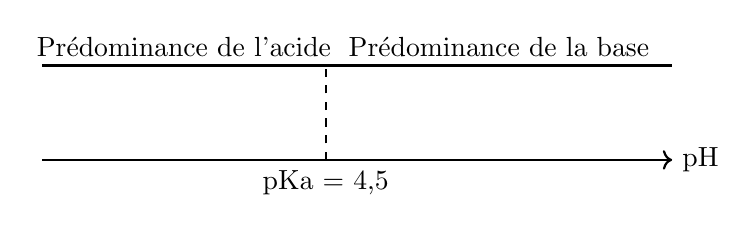
\begin{tikzpicture}[scale=0.8]
        \draw[->, thick] (0,0) -- (10,0) node[right] {pH};
        \draw[thick] (0,1.5) -- (10,1.5);
        \draw[thick, dashed] (4.5,0) node[below] {pKa = 4,5} -- (4.5,1.5);
        \node at (2.25,1.8) {Prédominance de l'acide};
        \node at (7.25,1.8) {Prédominance de la base};
    \end{tikzpicture}
    \end{center}
    }
\end{questionmult}

\begin{questionmult}{ibuprofene10}
    Déterminer la valeur du rapport des concentrations à l'équilibre de la forme acide et de la forme basique
    de l'ibuprofène dans le sang. Commenter.
    \begin{EnvQuadrillage}[NbCarreaux=20x4,Grille=Seyes,Marge=1]
    \end{EnvQuadrillage}
    \AMCOpen{}{
        \mauvaise[F]{NA}\scoring{b=0}
        \bonne[A1]{Raisonnement}\scoring{b=1}
        \bonne[A2]{Résultat}\scoring{b=1}
    }
    \explain{
    \begin{itemize}
        \item Le rapport des concentrations est donné par la relation de Henderson-Hasselbalch~:
        $$
        \frac{[\text{acide}]}{[\text{base}]} = 10^{pKa - pH}.
        $$
        \item Dans le sang (pH = 7,4), ce rapport est de $10^{4,5 - 7,4} \approx 0,0032$, ce qui signifie que la forme basique est largement prédominante.
    \end{itemize}
    }
\end{questionmult}


\end{document}
